Обучение игре в шахматы является одним из популярных подходов к формированию стратегического мышления.

В работе \cite{Adam2024} проведен анализ в соревнованиях проприетарного решение ChatGPT демонстрировал рейтинг Эло 1600,
соответствующий начальном уровню игрока в шахматы \cite{elo1967proposed}. Открытое решение \cite{feng2024chessgpt} использует архитектуру декодера для 


\begin{figure}[h]
    \centering
    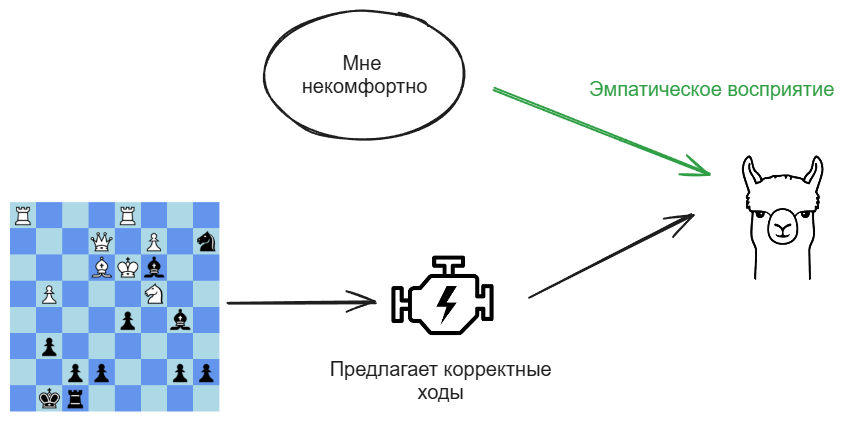
\includegraphics[width=0.5\textwidth]{assets/work/games/llama-chess.excalidraw.png}
    \caption{Планирование игры выполняется шахматным движком Stockfish. Языковой ассистент комментирует игру и следит за сложностью}
    \label{chess}
\end{figure}



Исходя из этого был подготовлен совместный подход, 
использующий открытый шахматный движок StockFish \cite{acher2016large} для ранжирования наилучшего хода. 

Таким образом, интеллектуальный ассистент отвечает за эмпатическое понимание пользователя и коррекцию сложности,
а шахматный движок предлагает ход согласно уровню игры.





